\documentclass[t,11pt]{article}
% A modifier selon la personne...
\NeedsTeXFormat{LaTeX2e}




\RequirePackage{geometry}
\usepackage{beamerarticle}
%\usepackage{boxedminipage,multicol,pifont}
\renewcommand{\d}{\textrm{d}}
\renewcommand{\baselinestretch}{1.3}
\newcommand{\longueur}{6cm}
\RequirePackage{amsmath,amssymb}
\RequirePackage{amsfonts}
\RequirePackage{graphicx}
%\RequirePackage{mesmacros}
\usepackage[T1]{fontenc} 
\usepackage[utf8]{inputenc}
\usepackage[frenchb]{babel}
\usepackage{pifont}
\usepackage{lmodern}

\RequirePackage{comment}
\RequirePackage{multicol}

\RequirePackage{colortbl}
\RequirePackage{fancybox}
\usepackage{colortbl}


\RequirePackage{tikz,tkz-tab,tkz-fct,tkz-base,tkz-euclide}
%\RequirePackage{tikz,tkz-base,tkz-euclide}

%\RequirePackage{graphe}
\RequirePackage{framed}

\usepackage{ulem}
\normalem


%%%ENTETES%%%
%%%%%%%%%%%
\newcommand{\entetedebut}{
{\noindent \textbf{PTSI2 -- 2019/2020 -- Maths} \hfill Lycée La Martinière-Monplaisir -- Lyon \vspace{2mm}}
\hrule
\begin{center} 
}
\newcommand{\entetedebutinfo}{
{\noindent \textbf{PTSI -- 2023/2024 -- Info} \hfill Lycée La Martinière-Monplaisir -- Lyon \vspace{2mm} }
\hrule
\begin{center} 
}

\newcommand{\entetefin}{
\end{center}
\hrule
\vspace*{0.5cm}
}

\newcommand{\entetedebutsnow}{
\begin{tikzpicture}[decoration=Koch snowflake]
\draw (0,0)--(12,0)node[midway,above]
}

\newcommand{\entetefinsnow}{
\draw decorate{ decorate{ decorate{ decorate{ (12,0)--(17,0) }}}};
\end{tikzpicture}
\vspace*{1cm}
}
%%% Lorqu'on utilise les entetes koch snowflake, il faut juste mettre tout le titre entre { } et un point-virgule à la fin, car on est dans un tikzpicture.
\newcommand{\entetecours}{
\entetedebut
\textbf{\textsf{\Large Ch \numero. \titre.}}
\entetefin
}
\newcommand{\entetecoursinfo}{
\entetedebutinfo
\textbf{\textsf{\Large Ch \numero. \titre.}}
\entetefin
}


\newcommand{\entete}{
\entetedebut
\textbf{\textsf{\Large \titre.}}
\entetefin
}
\newcommand{\enteteinfo}{
\entetedebutinfo
\textbf{\textsf{\Large \titre.}}
\entetefin
}


\newcommand{\entetetd}{
\entetedebut
\textbf{\textsf{\Large TD \numero. \titre.}}
\entetefin
}

\newcommand{\entetetp}{
\entetedebut
\textbf{\textsf{\Large TP \numero. \titre.}}
\entetefin
}

\newcommand{\entetetpinfo}{
\entetedebutinfo
\textbf{\textsf{\Large TP \numero. \titre.}}
\entetefin
}



\newcommand{\enteteindic}{
\entetedebut
\textbf{\textsf{\Large Indications et solutions pour le TD \numero.}}
\entetefin
}


\newcommand{\entetecor}{
\entetedebut
\textbf{\textsf{\Large Corrigés pour le TD \numero.}}
\entetefin
}


%%%%%%%%%%%%%%%%%%%%%%%%%%%%%%%%%%%%%%%
\parindent=0pt

\newlength{\myline}


\newcommand{\graphetext}[3]{
\setlength{\myline}{\linewidth}
\addtolength{\myline}{-1cm}
\addtolength{\myline}{-#1}
\begin{tabular}{ll}
\parbox[c]{#1}{\includegraphics[width=#1]{#2}}&
\parbox[c]{\myline}{#3}
\end{tabular}}
\newcommand{\tikztexte}[3]{
\setlength{\myline}{\linewidth}
\addtolength{\myline}{-1cm}
\addtolength{\myline}{-#1}
\begin{tabular}{ll}
\parbox[c]{#1}{#2}&
\parbox[c]{\myline}{#3}
\end{tabular}}
\newcommand{\textgraphe}[3]{
\setlength{\myline}{\linewidth}
\addtolength{\myline}{-.5cm}
\addtolength{\myline}{-#1}
\begin{tabular}{ll}
\parbox[c]{\myline}{#2}&
\parbox[c]{#1}{\includegraphics[width=#1]{#3}}
\end{tabular}}
\newcommand{\textetikz}[3]{
\setlength{\myline}{\linewidth}
\addtolength{\myline}{-.5cm}
\addtolength{\myline}{-#1}
\begin{tabular}{ll}
\parbox[c]{\myline}{#2}&
\parbox[c]{#1}{#3}
\end{tabular}}
\newcommand{\p}{\pause}


%%%NUMEROTATION DES PARTIES%%%
\renewcommand{\thesection}{\hspace{-0.6cm}\arabic{section}}
\renewcommand{\thesubsection}{\hspace{-0.4cm}\arabic{section}.\alph{subsection}}
\renewcommand{\thesubsubsection}{\hspace{0cm}\arabic{section}.\alph{subsection}.\roman{subsubsection}}

%% Pour l'entete prof

\usepackage{fancyhdr}
\pagestyle{fancy}
\renewcommand{\headrulewidth}{0pt}
\fancyhead[L]{}
\fancyhead[R]{}
\fancyhead[C]{\blanc{\texttt{\tiny{\phantom{version prof - }version prof -  version prof - version prof - version prof - version prof - version prof - version prof - version prof}}}}


\definecolor{shadecolor}{gray}{0.9}

\newcommand{\espace}[1]{\vspace*{#1cm}}
\newcommand{\commentaire}[1]{}
\newcommand{\pourmoi}[1]{}
\newcommand{\bonly}[1]{}
\newcommand{\bexcept}[1]{#1}

\newcommand{\eleveonly}[1]{#1}

\newcommand{\gris}[1]{\textcolor{white}{#1}}




%%%%%%%%%%%%%%%%%%Numerotation%%%%%%%%%%%%%%%%%%

\renewcommand{\labelenumi}{\textbf{\arabic{enumi}${}^\circ$)}}
\renewcommand{\labelenumii}{\textbf{\alph{enumii})}}
%\renewcommand{\thesection}{\Roman{section}}
%\renewcommand{\thesubsection}{\Alph{subsection})}
%\renewcommand{\thesubsubsection}{\arabic{subsubsection})}

%\renewenvironment{itemiz}%
%{\begin{itemize}\renewcommand{\labelitemi}{\ding{51}}}
%{\end{itemize}}


%\newenvironment{itemiz}[1][84]% 117 81 71
%{\begin{dinglist}{#1}}
%{\end{dinglist}}

%\newenvironment{itemiz}[1][]
%{\begin{itemize} \itemsep5pt 
 %\renewcommand{\labelitemi}{\bubul}}
%{\end{itemize}}

\newenvironment{itemiz}[1][]%
{ \begin{list}%
	{\bubul}%
	{%\setlength{\labelwidth}{30pt}%
	 \setlength{\leftmargin}{20pt}%
	 \setlength{\itemsep}{4pt}}}%
{ \end{list} }


%%%%%%%%%%%%%%%%%%%%%%%Les encadrés%%%%%%%%%%%%%%%%
\newenvironment{python}
{\vspace{-0.2cm}\begin{shaded}\ttfamily}
{\normalfont\end{shaded}\vspace{0.2cm}}

\newenvironment{pythonshell}
{\begin{shaded}
\textit{Python shell}\\
\ttfamily}
{\normalfont\end{shaded}\vspace{0.2cm}}




%\newenvironment{defn}[1][]{\vspace{.2cm}
%\begin{minipage}{\linewidth}
%{\bf Définition\vphantom{p} : #1}
%\newline
%\noindent
%\begin{boxedminipage}{\linewidth}}{
%\end{boxedminipage}\vspace{.5cm}\end{minipage}}

%\newenvironment{defn}[1][]{\vspace{.2cm}
%\begin{minipage}{\linewidth}
%{\bf Définition\vphantom{p} : #1}
%\newline
%\noindent
%\begin{boxedminipage}{\linewidth}}{
%\vspace{.05cm}\end{boxedminipage}\vspace{0.2cm}\end{minipage}}

\newcommand{\debutprop}{\newline
\hspace*{5mm}
\begin{tikzpicture}
  \node[rectangle,inner sep=0pt,outer sep=10pt]%
  (A)  \bgroup
    \begin{minipage}{0.9\linewidth}
    }
    
\newcommand{\finprop}{
    \end{minipage}
    \egroup;
\draw (A.north west) -- (A.south west) ;
\draw (A.south west) -- (A.south east) ;
%\draw (A.north west) -- (A.north east) ;
%\draw (A.north east) -- (A.south east) ;
\end{tikzpicture}\\
}

\newenvironment{defn}[1][]
{\textbf{Définition\vphantom{p} : #1}\debutprop
      }
     {\finprop
}


%\newenvironment{cor}[1][]{\vspace{.2cm}
%\begin{minipage}{\linewidth}
%{\bf Corollaire\vphantom{p} : #1}
%\newline
%\noindent
%\begin{boxedminipage}{\linewidth}}{
%\vspace{.05cm}\end{boxedminipage}\vspace{0.2cm}\end{minipage}}

\newenvironment{cor}[1][]
{\textbf{Corollaire\vphantom{p} : #1}\debutprop}
     {\finprop}

%\newenvironment{lemme}[1][]{\vspace{.2cm}
%\begin{minipage}{\linewidth}
%{\bf Lemme\vphantom{p} : #1}
%\newline
%\noindent
%\begin{boxedminipage}{\linewidth}}{
%\vspace{.05cm}\end{boxedminipage}\vspace{0.2cm}\end{minipage}}

\newenvironment{lemme}[1][]
{\textbf{Lemme\vphantom{p} : #1}\debutprop}
     {\finprop}


%\newenvironment{theo}[1][]{\vspace{.2cm}
%\begin{minipage}{\linewidth}
%{\bf ThéorÚme \vphantom{p}: #1}
%\newline
%\noindent
%\begin{boxedminipage}{\linewidth}}{
%\vspace{.05cm}\end{boxedminipage}\vspace{0.2cm}\end{minipage}}

\newenvironment{theo}[1][]
{\textbf{Théorème\vphantom{p} : #1}\debutprop}
     {\finprop}
     
     \newenvironment{theodefn}[1][]
{\textbf{Théorème-définition\vphantom{p} : #1}\debutprop}
     {\finprop}


%\newenvironment{propdef}[1][]{\vspace{.2cm}
%\begin{minipage}{\linewidth}
%{\bf Proposition et définition : #1}
%\newline
%\noindent
%\begin{boxedminipage}{\linewidth}}{
%\vspace{.05cm}\end{boxedminipage}\vspace{0.2cm}\end{minipage}}

\newenvironment{propdef}[1][]
{\textbf{Proposition-définition\vphantom{p} : #1}\debutprop}
     {\finprop}

%\newenvironment{prop}[1][]{\vspace{.2cm}\noindent
%\begin{minipage}{\linewidth}{\bf Proposition : #1}
%\newline
%\noindent
%\begin{boxedminipage}{\linewidth}}{
%\vspace{.05cm}\end{boxedminipage}\vspace{0.2cm}\end{minipage}}

\newenvironment{prop}[1][]
{\textbf{Proposition\vphantom{p} : #1}\debutprop}
     {\finprop}

\newenvironment{rem}[1][]{\vspace{.2cm}\noindent\begin{minipage}{\linewidth}{\bf Remarque : #1}\newline\noindent}{\end{minipage}\vspace{.5cm}}
\newenvironment{meth}[1][]{\vspace{.2cm}\noindent\begin{minipage}{\linewidth}{\bf Méthode : #1}\newline\noindent}{\end{minipage}\vspace{.5cm}}
\newenvironment{rems}[1][]{\vspace{.2cm}\noindent\begin{minipage}{\linewidth}{\bf Remarques : #1}\noindent}{\end{minipage}\vspace{0.5cm}}
\newenvironment{remnum}[1]{\vspace{.2cm}\noindent\begin{minipage}{\linewidth}{\bf Remarque #1 : }\newline\noindent}{\end{minipage} \vspace{.5cm}}
\newenvironment{exe}[1][]{\vspace{0.2cm}\noindent\begin{minipage}{\linewidth}{\bf Exemple : #1}\newline\noindent}{\end{minipage}\vspace{.5cm}}
\newenvironment{exes}[1][]{\vspace{0.2cm}\noindent\begin{minipage}{\linewidth}{\bf Exemples : #1}\noindent}{\end{minipage}\vspace{0.5cm}}
\newenvironment{exenum}[1]{\vspace{.2cm}\noindent\begin{minipage}{\linewidth}{\bf Exemple #1 : }\newline\noindent}{\end{minipage}\vspace{.5cm}}
\newenvironment{nota}[1][]{\vspace{.2cm}\noindent\begin{minipage}{\linewidth}{\bf Notation : #1}\newline\noindent}{\end{minipage}\vspace{.5cm}}
\newcounter{ndem}
\setcounter{ndem}{0}
\newcommand{\dem}{\stepcounter{ndem}{\includegraphics{crayon5} \ \textbf{Démonstration} \thendem }\vspace{.5cm}}



%%% numerotation des questions exo
\newcounter{cexo}
\newenvironment{qexo}{
\refstepcounter{cexo}
\vspace{3 pt}
\noindent
\begin{minipage}[t]{0.15\textwidth}
\textbf{\noindent Question \arabic{cexo}. }
\end{minipage}\noindent
\begin{minipage}[t]{0.85\textwidth}}{\vspace{3 pt}
\end{minipage}}%\vspace{2 pt}


\usepackage{multicol}
\usepackage{ulem}
\normalem

\parindent=0pt

\RequirePackage{framed}

\graphicspath{{images_archi_materielle/}{images_archi_logicielle/}}
\newcommand{\FIG}[1]{\textsc{Figure} {\upshape\ref{#1}}}
\usepackage{numprint} %affichage de nombres correctement avec \numprint{}

%\usepackage{picins}    %permet d'insérer une image à coté d'un texte \parpic[r]{\includegraphics{}}texte...
\usepackage{tikz}
\usetikzlibrary{calc}
% Unités
\usepackage[locale = FR]{siunitx}
\sisetup{inter-unit-product = \ensuremath{{}\cdot{}}}
\usepackage{numprint} %affichage de nombres correctment avec \numprint{}
\usepackage{multirow}
\definecolor{gris_c}{gray}{0.9}
\definecolor{gris_f}{gray}{0.25}
\definecolor{gris_tc}{gray}{0.96}
\definecolor{gris_ttc}{gray}{0.98}

%%% activite
\newenvironment{activite}[1][\hsize]%
{%
    \def\FrameCommand%
    {%
\rotatebox{90}{\textit{\textsf{REMARQUE}}} 
        {\color{blue}\vrule width 3pt}%
        \hspace{0pt}%must no space.
        \fboxsep=\FrameSep\colorbox{gris_c}%
    }%
    \MakeFramed{\hsize#1\advance\hsize-\width\FrameRestore}%
}%
{\endMakeFramed}%


%%% objectif
\newenvironment{objectif}[1][\hsize]%
{%
    \def\FrameCommand%
    {%
\rotatebox{90}{\textit{\textsf{OBJECTIF}}} 
        {\color{blue}\vrule width 3pt}%
        \hspace{0pt}%must no space.
        \fboxsep=\FrameSep\colorbox{gris_c}%
    }%
    \MakeFramed{\hsize#1\advance\hsize-\width\FrameRestore}%
}%
{\endMakeFramed}%

%%%%exos TP Info



\newtheorem{Exc}{Exercice}
\def\exotp#1{\futurelet\testchar\MaybeOptArgmyexoo}
\def\MaybeOptArgmyexoo{\ifx[\testchar \let\next\OptArgmyexoo
                        \else \let\next\NoOptArgmyexoo \fi \next}
\def\OptArgmyexoo[#1]{\begin{Exc}[#1]\normalfont}
\def\NoOptArgmyexoo{\begin{Exc}\normalfont}
\newcommand{\finexotp}{\end{Exc}}

\theoremstyle{definition}
\newtheorem{exo}{Exercice}

\usetikzlibrary{decorations.fractals}
\usetikzlibrary{matrix}

\newcommand{\cache}[1]{\phantomchoix{#1}\hspace{1.5cm}}
\newcommand{\Cache}[1]{\vspace*{0.2cm}\phantomchoix{\begin{minipage}{\linewidth}{#1}\end{minipage}}\vspace*{0.5cm}}

\newcommand{\indente}{\hspace*{1cm}}
\newcommand{\invite}{{>}{>}{>} }


\renewcommand{\vec}[1]{\overrightarrow{#1}}
\newcommand{\B}{\mathcal{B}}
\renewcommand{\P}{\mathcal{P}}
\renewcommand{\epsilon}{\varepsilon}
\newcommand{\A}{\mathcal{A}}
\newcommand{\re}{\mathcal{R}}

\newcommand{\un}{{1\!\mbox{l}}}
\newcommand{\E}{\mathbb{E}}
\newcommand{\R}{\mathbb{R}}
\newcommand{\Z}{\mathbb{Z}}
\newcommand{\Q}{\mathbb{Q}}
\newcommand{\N}{\mathbb{N}}
\newcommand{\C}{\mathbb{C}}
\newcommand{\U}{\mathbb{U}}
\newcommand{\cc}{\small{\mathbb{c}}}
\newcommand{\F}{\mathcal{F}}
\newcommand{\K}{\mathbb{K}}
% Commande \tend :
% bla \tend{n}{l} bli :
%
%      bla   ->   bli
%          n -> l
%
%\newcommand{\tend}[2]{{\atop\stackrel{\displaystyle\longrightarrow}{\scriptstyle{{#1} \rightarrow {#2}}}}}
\newcommand{\tend}[2]{\underset{#1 \rightarrow #2}{\longrightarrow}}
\renewcommand{\o}[1]{\underset{#1}{o}}
%\renewcommand{\O}[1]{\underset{#1}{O}}
\DeclareMathOperator{\Det}{Det}

\newcommand{\Max}[1]{\underset{#1}{\max}\ }
\newcommand{\Min}[1]{\underset{#1}{\min}\ }
\newcommand{\Inf}[1]{\underset{#1}{\inf}\ }
\newcommand{\Sup}[1]{\underset{#1}{\sup}\ }
\newcommand{\Lim}[1]{\underset{#1}{\lim}\ }
\newcommand{\Sim}[1]{\underset{#1}{\sim}\ }
\def\det{\mathop{\operator@font det}\nolimits}
\def\Tr{\mathop{\operator@font Tr}\nolimits}
\def\Card{\mathop{\operator@font Card}\nolimits}
%\def\Ker{\mathop{\operator@font Ker}\nolimits}
\newcommand{\Ker}{\textrm{Ker}}
\newcommand{\Vect}{\textrm{Vect}}
\def\rg{\mathop{\operator@font rg}\nolimits}
\def\Im{\mathop{\operator@font Im}\nolimits}
\def\Re{\mathop{\operator@font Re}\nolimits}
%\def\Arg{\mathop{\operator@font Arg}\nolimits}
\def\Argsh{\mathop{\operator@font Argsh}\nolimits}
\def\Argch{\mathop{\operator@font Argch}\nolimits}
\def\Argth{\mathop{\operator@font Argth}\nolimits}
%\def\cotan{\mathop{\operator@font cotan}\nolimits}
\def\Arctan{\mathop{\operator@font Arctan}\nolimits}
\def\Arccos{\mathop{\operator@font Arccos}\nolimits}
\def\Arcsin{\mathop{\operator@font Arcsin}\nolimits}
\def\Argcoth{\mathop{\operator@font Argcoth}\nolimits}
%\def\sh{\mathop{\operator@font sh}\nolimits}
\def\coth{\mathop{\operator@font coth}\nolimits}
\def\tanh{\mathop{\operator@font th}\nolimits}
%\def\ch{\mathop{\operator@font ch}\nolimits}
\def\div{\mathop{\operator@font div}\nolimits}
\def\rot{\mathop{\overrightarrow{\operator@font rot}}\nolimits}
\def\grad{\mathop{\overrightarrow{\operator@font grad}}\nolimits}

\def\card{\mathop{\operator@font card}\nolimits}
\newcommand{\scal}[2]{\langle #1 | #2 \rangle}
\newcommand{\norme}[1]{\| #1 \|}
%\newcommand{\ang}[1]{\sphericalangle #1}

\newcommand{\fonc}[4]{\begin{array}[t]{rcl}
#1&\rightarrow&#2\\
#3&\mapsto&#4\end{array}}

%\newcommand{\soupoint}[1]{\d}
\renewcommand{\d}{\,\textrm{d}}
%\renewcommand{\d}{\operatorname{d}\!}
\newcommand{\der}[3][]{\dfrac{\textrm{d}^{#1} #2}{\textrm{d} #3^{#1}}}
\newcommand{\derpar}[3][]{\dfrac{\partial^{#1} #2}{\partial #3^{#1}}}
\newcommand{\dercroise}[3]{\dfrac{\partial^{2}#1}{\partial#2\partial#3}}
\newcommand{\doubleint}{\int\!\!\!\int}
\newcommand{\tripleint}{\int\!\!\!\int\!\!\!\int}

\newcommand{\D}[1]{\displaystyle{#1}}

\renewcommand{\bar}{\overline}




%%%Delphine%%%
%%%COMMANDES PRATIQUES%%%
%%%GENERAL%%%
\newcommand{\bubul}{$\bullet$ }
\newcommand{\qqsoit}{\forall \,}
\newcommand{\ilex}{\exists \,}
\newcommand{\di}{\displaystyle}
\newcommand{\ep}{\varepsilon}
\renewcommand{\l}{\lambda}
\newcommand{\ssi}{\Longleftrightarrow}
%\newcommand{\sensdirect}{\fbox{$\Rightarrow$} }
%\newcommand{\sensindirect}{\fbox{$\Leftarrow$} }
\newcommand{\li}{\begin{itemize}}
\newcommand{\finli}{\end{itemize}}
\newcommand{\syst}{\left\{\begin{array}{l}}
\newcommand{\finsyst}{\end{array} \right.}
\newcommand{\va}{|}
\newcommand{\plrs}{\begin{eqnarray*}}
\newcommand{\finplrs}{\end{eqnarray*}}
\newcommand{\Arg}{\text{Arg}}
\newcommand{\ent}[1]{\left\lfloor #1\right\rfloor}

%%%PROBAS%%%
%\DeclareMathOperator{\card}{Card}
%\newcommand{\E}{\mathbb{E}}    
%\renewcommand{\P}{\mathbb{P}}  
\newcommand{\cov}{\text{cov}}  

%%%ANALYSE%%%
\providecommand{\abs}[1]{\left\lvert#1\right\rvert} %valeur absolue
\providecommand{\fonction}[5]
    {\begin{array}[t]{cccl}#1  : & #2&\rightarrow&#3\\{} & #4&\mapsto&#5\end{array}}
\providecommand{\eq}[2]{\underset{#1 \rightarrow #2}{\sim}}
\providecommand{\tend}[2]{\underset{#1 \rightarrow #2}{\longrightarrow}}
\providecommand{\limite}[2]{\displaystyle \lim_{#1 \rightarrow #2}}
\providecommand{\dl}[2]{\underset{#1 \rightarrow #2}{=}}
%\renewcommand{\d}{\operatorname{d}}
\newcommand{\drond}{\partial}
\renewcommand{\i}{\operatorname{i}}
\newcommand{\ch}{\operatorname{ch}}
\newcommand{\sh}{\operatorname{sh}}
\renewcommand{\th}{\operatorname{th}}
\newcommand{\cotan}{\operatorname{cotan}}
\renewcommand{\arctan}{\operatorname{Arctan}}
\renewcommand{\arcsin}{\operatorname{Arcsin}}
\renewcommand{\arccos}{\operatorname{Arccos}}
\newcommand{\argth}{\operatorname{argth}}
\newcommand{\argsh}{\operatorname{argsh}}
\newcommand{\argch}{\operatorname{argch}}
\renewcommand{\Re}{\text{Re}}
\renewcommand{\Im}{\text{Im}}

%%%ALGEBRE%%%
\providecommand{\norm}[1]{\left\rVert#1\right\rVert} %norme
\providecommand{\sdo}[0]{\text{\odplus}} % somme directe orthogonale
\renewcommand{\ker}{\operatorname{Ker}}
%\newcommand{\Ker}{\operatorname{Ker}}
%\renewcommand{\o}{\operatorname{o}}
\renewcommand{\O}{\operatorname{O}}
\newcommand{\trans}{\,{}^{\text{t}}} % transposée
\DeclareMathOperator{\tr}{tr}  %trace
%\DeclareMathOperator{\im}{\text{Im}}
\newcommand{\im}{\operatorname{Im}}
\DeclareMathOperator{\id}{id}
\providecommand{\mat}[1]{\underset{#1}{\text{mat}}}
\DeclareMathOperator{\vect}{\text{Vect}}
%\DeclareMathOperator{\rg}{\text{rg}}


%%%MAPLE%%%
\newenvironment{prog}{ \color{red}\ttfamily}{\color{black}}
\newcommand{\maple}{\begin{prog}}
\newcommand{\finmaple}{\end{prog}}
\newenvironment{reponse}{ \begin{center}  \color{blue} \em}{\end{center}\color{black}}
\newcommand{\rep}{\begin{reponse}}
\newcommand{\finrep}{\end{reponse}}


%%%GEOMETRIE%%%
\providecommand{\vecteur}[1]{\overrightarrow{#1}}

%%DIVERS%%
%\newcommand{\s}{ $ }
%\newcommand{\ds}{ $$ }
\newcommand{\itbul}{\item[\bubul]}

%\usepackage{tikz,tkz-tab}
%\usepackage[babel=true,kerning=true]{microtype}

\tikzset{math3d/.style={x={(-0.353cm,-0.353cm)},z={(0cm,1cm)},y={(1cm,0cm)}}}

\tikzset{
xmin/.store in=\xmin, xmin/.default=-3, xmin=-3,
xmax/.store in=\xmax, xmax/.default=3, xmin=3,
ymin/.store in=\ymin, ymin/.default=-3, ymin=-3,
ymax/.store in=\ymax, ymax/.default=-3, ymax=-3,
}
\newcommand{\grille}{\draw[help lines] (\xmin,\ymin) grid (\xmax,\ymax);}

\newcommand{\axes}{%
\draw[->] (\xmin,0)--(\xmax,0);
\draw[->] (0,\ymin)--(0,\ymax);
\draw[->][very thick] (0,0)--(1,0);
%\draw (1 , 0) node[below] {$1$};
%\draw (0.5 , 0) node[below] {$\vec{i}$};
\draw (0.5 , 0) node[below] {$\vec{\imath}$};
\draw[->] [very thick](0,0)--(0,1);
%\draw (0,0.5) node[left] {$\vec{j}$};
\draw (0 , 0.5) node[left] {$\vec{\jmath}$};
%\draw (0,1) node[left] {$1$};
%\draw (0,0) node[below left]{$O$};
}

\newcommand{\axesbis}{%
\draw[->] (\xmin,0)--(\xmax,0)node[below]{$x$};
\draw[->] (0,\ymin)--(0,\ymax)node[left]{$y$};
}

\newcommand{\fenetre}
{\clip (\xmin,\ymin) rectangle (\xmax,\ymax);}

\newcommand{\repere}{%
\tikzset{xaxe style/.style={-}}
\tikzset{yaxe style/.style={-}}
\tkzInit[xmin=\xmin,xmax=\xmax,ymin=\ymin,ymax=\ymax]
\tkzDrawX[noticks]\tkzDrawY[noticks]
\tkzRep
}

\newcommand{\attention}{\raisebox{-2pt}{\includegraphics[width=5mm]{/Users/Delphine/1.BOULOT/2019_2020_PTSI_info/attention}}\ }

\geometry{a4paper,top=2cm,bottom=2cm,left=2cm,right=2cm}

% A modifier pour chaque chapitre...
\newcommand{\titre}{Les algorithmes de tris}
\newcommand{\numero}{13}

% Prof ou élève...
% prof : 
%\newcommand{\phantomchoix}[1]{\textcolor{red}{#1}}
%\newcommand{\blanc}[1]{\textcolor{red}{#1}}
% eleve : 
\newcommand{\phantomchoix}[1]{\phantom{#1}}
\newcommand{\blanc}[1]{\textcolor{white}{#1}}

\renewcommand{\cache}[1]{\phantomchoix{#1}\hspace*{0.1mm}}

%%% utilisation des algorithmes
\usepackage{algorithm}
\usepackage{algorithmic}
\renewcommand{\algorithmicrequire} {\textbf{\textsc{Entrées:}}}
\renewcommand{\algorithmicensure}  {\textbf{\textsc{Sorties:}}}
\renewcommand{\algorithmicwhile}   {\textbf{tantque}}
\renewcommand{\algorithmicdo}      {\textbf{faire}}
\renewcommand{\algorithmicendwhile}{\textbf{fin tantque}}
\renewcommand{\algorithmicend}     {\textbf{fin}}
\renewcommand{\algorithmicif}      {\textbf{si}}
\renewcommand{\algorithmicendif}   {\textbf{finsi}}
\renewcommand{\algorithmicelse}    {\textbf{sinon}}
\renewcommand{\algorithmicthen}    {\textbf{alors}}
\renewcommand{\algorithmicfor}     {\textbf{pour}}
\renewcommand{\algorithmicforall}  {\textbf{pour tout}}
\renewcommand{\algorithmicdo}      {\textbf{faire}}
\renewcommand{\algorithmicendfor}  {\textbf{fin pour}}
\renewcommand{\algorithmicloop}    {\textbf{boucler}}
\renewcommand{\algorithmicendloop} {\textbf{fin boucle}}
\renewcommand{\algorithmicrepeat}  {\textbf{répéter}}
\renewcommand{\algorithmicuntil}   {\textbf{jusqu'à}}

\floatname{algorithm}{Algorithme}

\let\mylistof\listof
\renewcommand\listof[2]{\mylistof{algorithm}{Liste des algorithmes}}

% pour pallier au problème de niveau des algos
\makeatletter
\providecommand*{\toclevel@algorithm}{0}
\makeatother

\begin{document}
\entetecoursinfo


\begin{framed}
\underline{Objectifs :}
\begin{itemize}
\item[-] Comprendre et analyser un algorithme de tri ;
\item[-] Évaluer la complexité d'un algorithme de tri ;
\item[-] Comparer différents algorithmes de tri.
\end{itemize}
\end{framed}



\section{Présentation}

\begin{minipage}{.65\textwidth}%
Un algorithme de tri est un algorithme qui permet d'organiser une collection d'objets selon un ordre déterminé. Le tri permet notamment de faciliter les recherches ultérieures d'un élément dans une liste (recherche dichotomique).
On s'intéresse ici à des méthodes de tri d'une liste de valeurs numériques. Celle-ci est implémentée sous la forme d'un tableau à une dimension.

\end{minipage}%
\hfill
\begin{minipage}{.3\textwidth}%

\includegraphics[width=\textwidth]{images/cartes.png}
\end{minipage}

%---------------------------------------------------------------------------
\section{Complexité d'un algorithme de tri}
%---------------------------------------------------------------------------
\subsection{Définitions}
%---------------------------------------------------------------------------
\begin{framed}
\noindent
\underline{Ordre de grandeur} :
Soient $f$ et $g$ deux fonctions positives d'une même variable entière $n$. La fonction $f$ est dite avoir un ordre de grandeur au plus égal à celui de la fonction $g$ s'il existe un entier
strictement positif $k$ et un entier $N$ tels que, pour tout $n \geq N$, on ait $f(n) \leq k \times g(n)$. 
On écrira $f = O(g)$. Par exemple, les fonctions $f(n) = 3 n^{2} - 5 n + 4$ et
$g(n) = n^{2}$ ont même ordre de grandeur.\\
\\
\noindent
\underline{Complexité} :
On considère un algorithme $A$. On appelle complexité de $A$ tout ordre de grandeur du
nombre d'opérations élémentaires effectuées pendant le déroulement de l'algorithme. On
exprime ce nombre d'opérations en fonction de paramètres entiers associés aux instances à
traiter ; on pourra par exemple exprimer la complexité d’un tri en fonction du nombre de
données à trier. 
\end{framed}

\noindent
Néanmoins, il se peut qu’avec deux jeux de données différents correspondant
aux mêmes paramètres, le nombre d’opérations effectuées ne soit pas le même. Par exemple,
un algorithme de tri pourra être plus rapide s’il s’agit de trier des données déjà triées que s’il
s’agit de données très désordonnées. On peut alors s’intéresser à :

\begin{itemize}
\item la complexité \textbf{dans le pire des cas} : les paramètres avec lesquels on exprime la
complexité étant fixés, on considère le plus grand nombre d’opérations
élémentaires effectuées sur l’ensemble des instances correspondant à ces
paramètres ; on cherche ainsi un majorant de la complexité qui puisse être atteint
dans certains cas ; c’est ce qu’on fait le plus généralement ;
\item la complexité \textbf{dans le meilleur des cas} : les paramètres avec lesquels on exprime la
complexité étant fixés, on considère le plus petit nombre d’opérations élémentaires
effectuées sur l’ensemble des instances correspondant à ces paramètres ; cette
complexité peut venir compléter la précédente mais ne sera jamais suffisante pour
l’utilisateur ;
\item la complexité \textbf{en moyenne} \textit{(pour information)}: les paramètres avec lesquels on exprime la complexité
étant fixés, il faut alors faire la moyenne des nombres d’opérations élémentaires effectuées, moyenne portant sur tous les jeux de données correspondant à ces paramètres. Ce calcul est généralement difficile et souvent même délicat à
formuler car il faut connaître la probabilité de chacun des jeux de données pour effectuer un calcul pertinent de cette moyenne.
\end{itemize}

%---------------------------------------------------------------------------
\subsection{Illustration}
%---------------------------------------------------------------------------
\noindent
Il existe plusieurs types d'algorithmes de tri que l'on peut classer en comparatifs (ce que l'on verra dans ce cours) et non comparatifs.
Un algorithme comparatif est basé sur des comparaisons successives entre les données pour déterminer la permutation correspondant à l'ordre croissant des données.
On va chercher ici à évaluer la complexité théorique des tris comparatifs en se basant sur le nombre de comparaisons.
\noindent
Prenons un exemple:
on considère un algorithme pour
trier trois données a, b et c décrit par l’arbre ci-dessous ; cet algorithme correspond au fonctionnement du tri insertion que nous verrons plus loin :
\begin{center}
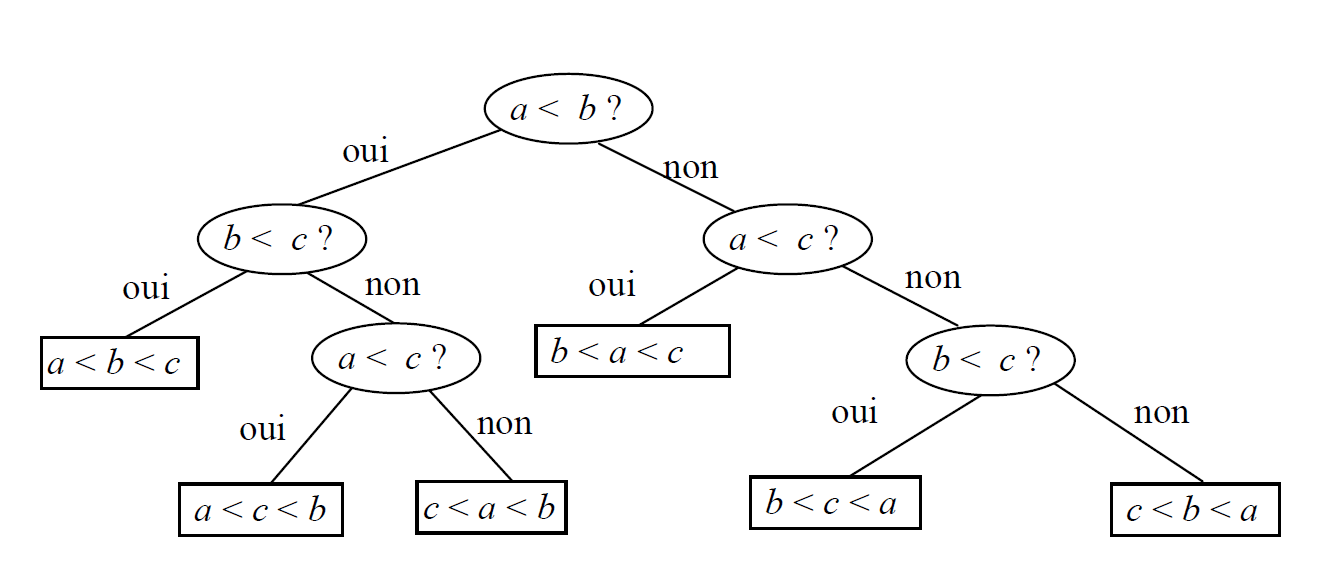
\includegraphics[width=.85\textwidth]{images/C2.png}
\end{center}

\noindent
Cet arbre signifie : la première comparaison faite est « a < b ? ». Si la réponse est oui, la
comparaison suivante est « b < c ? », si la réponse est non c'est « a < c ? ». Lorsqu’une permutation est déterminée, on est dans ce que l'on appelle une feuille de l'arbre. On voit qu'on peut avoir plus
ou moins de chance ; pour deux des permutations, on fait deux comparaisons, pour les quatre
autres, on fait trois comparaisons. Le plus grand nombre de comparaisons est 3, le meilleur est
2 et le nombre moyen de comparaisons est : $(2 \times 2 + 4 \times 3) / 6 \approx 2,67$.

\newpage

\section{Tri par Insertion}
\subsection{Principe}

Le tri par insertion est le tri que l'on effectue naturellement, par exemple pour trier un jeu de cartes.

Soit un jeu de n cartes. On prend la première dans une main. On saisit la seconde carte et on l'insère avant ou après la première selon le cas.
A l'étape « i », la $i^{ème}$ carte est insérée à sa place dans le paquet déjà trié.\\
Pour cela, on peut :
\begin{itemize}
\item soit partir de la fin du tas déjà trié et s'arrêter si on rencontre une carte plus petite que la $i^{ème}$ (méthode 1) ;
\item 	soit partir du début du tas déjà trié et s'arrêter lorsqu'on rencontre une carte plus grande que la $i^{ème}$ (méthode 2).
\end{itemize}
	
Le paquet contient alors « i » cartes triées. On procède ainsi de suite jusqu'à la dernière carte.

Ce tri s'effectue en place, c'est-à-dire qu'il ne demande pas d'autre tableau que celui que l'on trie. 
Son coût en mémoire est donc constant si on ne compte pas la place occupée par les données.

\vspace*{0.5cm}
\texttt{Exemple} : L'objectif de cet exemple est de trier "à la main" la liste L=\verb![!7,6,3,5,4,2,1,8\verb!]! par insertion.
On choisira comme clef (nouvel élément à trier) le premier élément non trié. 
\begin{python}

\vspace*{13cm}

\end{python}

\subsection{Algorigramme du tri par insertion}

L'algorithme proposé présente une comparaison avec, en premier, l'élément se situant à droite de la partie triée (méthode 1).

\begin{minipage}{.45\textwidth}%
\begin{center}
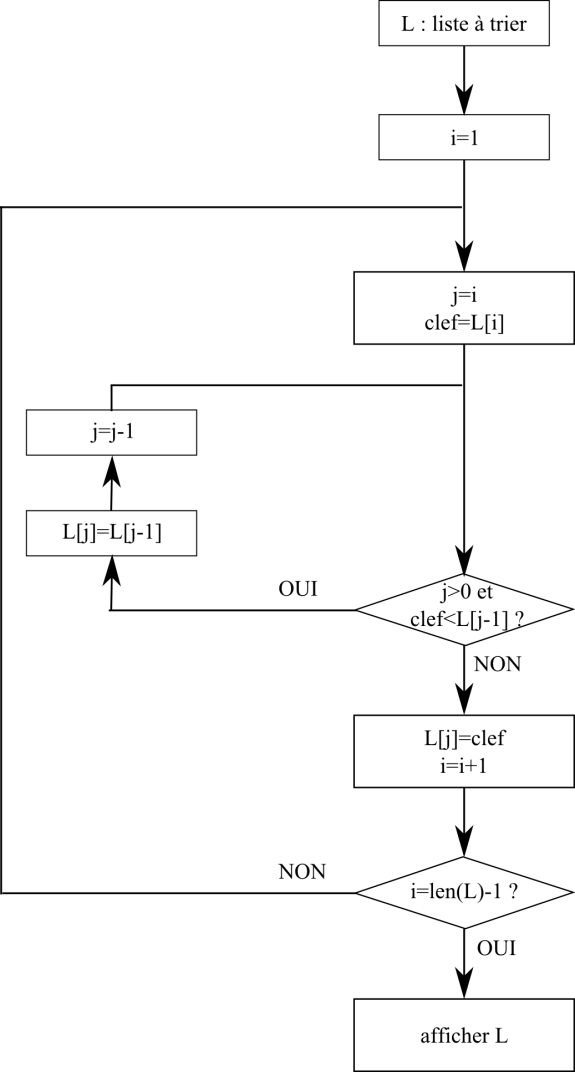
\includegraphics[width=1\textwidth]{images/algorigramme_insertion.png}
\end{center}
\end{minipage}%
\hfill
\begin{minipage}{.5\textwidth}%
\vspace*{0.6cm}
\begin{python}
Commentaires
\vspace*{13cm}
\end{python}
\end{minipage}

\vspace{-0.2cm}
\subsection{Implémentation en python}
\vspace{-0.2cm}
\begin{python}
Tri par insertion :\\
\textbf{def} tri\_Insertion(t:list)-> \textbf{None} :\\
\indente $'''$ \textit{Trie la liste t\\
\indente Entrée : Une liste \texttt{t}\\
\indente Sortie : La liste est modifiée mais n'est pas renvoyée} $'''$\\
\indente \textbf{for} i \textbf{in} range (1 , len(t)) :\\
\indente \indente cle = t[i]\\
\indente \indente k = i-1\\
\indente \indente \textbf{while} ( k >= 0 \textbf{and} t[k] > cle ) :\\
\indente \indente \indente t[k+1]=t[k]\\
\indente \indente \indente k=k-1\\
\indente \indente t[k+1] = cle

\end{python}

%---------------------------------------------------------------------------
\section{Tri rapide (quicksort par Tony Hoare - 1960)}
%---------------------------------------------------------------------------
\subsection{Principe}
%---------------------------------------------------------------------------
\noindent
L'algorithme fait partie de la catégorie des algorithmes « diviser pour régner ».\\
\'A chaque appel de la fonction tri, on choisit une valeur "pivot", par exemple le dernier élément.
On effectue ensuite une partition des éléments à trier :
\begin{itemize}
\item un premier groupe est constitué de valeurs inférieures au pivot ;
\item un deuxième avec les valeurs supérieures.
\end{itemize}
Ainsi à chaque appel de la fonction, le nombre de données à traiter est diminué de un. C'est-à-dire que l'on ne traite plus l'élément appelé « pivot » dans les appels ultérieurs de fonction, il est placé à sa place définitive dans le tableau.

\subsection{Algorigramme du tri rapide}

\begin{minipage}{.5\textwidth}%
\begin{center}
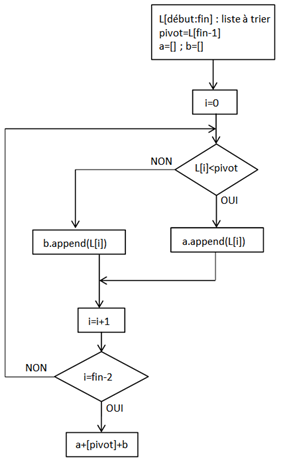
\includegraphics[width=1\textwidth]{images/algorigramme_rapide.png}
\end{center}
\end{minipage}%
\hfill
\begin{minipage}{.45\textwidth}%
\vspace*{0.6cm}
\begin{python}
Commentaires
\vspace*{13cm}
\end{python}
\end{minipage}


\newpage
\subsection{Implémentations en python}

\begin{python}
Tri rapide (méthode avec l'utilisation de deux listes de stockage) :\\
\textbf{def} tri\_rapide(t:list)-> list :\\
\indente $'''$ \textit{Trie la liste t par une méthode récursive\\
\indente Entrée : Une liste \texttt{t}\\
\indente Sortie : La liste est modifiée} $'''$\\
\indente \textbf{if} len(t) < 2 :\\
\indente \indente \textbf{return} (t)\\
\indente \textbf{else} :\\
\indente \indente x = t[-1]\\
\indente \indente a=[]\\
\indente \indente b=[]\\
\indente \indente \textbf{for} i \textbf{in} range (0,len(t)-1) :\\
\indente \indente \indente \textbf{if} t[i] < x :\\
\indente \indente \indente \indente a.append(t[i])\\
\indente \indente \indente \textbf{else} :\\ 
\indente \indente \indente \indente b.append(t[i])\\
\indente \indente \textbf{return} (tri\_rapide(a) + [x] + tri\_rapide(b))
\end{python}


\textit{Remarque} :\\
Certains algorithmes de tri rapide prennent pour « pivot » le premier élément, la valeur moyenne du premier et du dernier, ou un positionnement aléatoire dans le tableau. Pour se placer dans le meilleur des cas pour chaque segment de tableau, il faut prendre pour pivot la valeur médiane du tableau de valeurs. Le problème est que cette recherche de pivot idéal a aussi un « coût ».


\section{Méthodes de Python}

\subsection{sort et sorted}
Les listes Python ont une méthode native \texttt{list.sort()} qui modifie les listes elles-mêmes et renvoie \textbf{None}.
\vspace{-0.5cm}
\begin{pythonshell}
\invite a=[25,94,89,113,67]\\
\invite a.sort()\\
\invite a\\
\verb![!25,67,89,94,113\verb!]!
\end{pythonshell}

Il y a également une fonction native \texttt{sorted()} qui construit une nouvelle liste triée depuis un itérable (liste de listes, tuple, dictionnaires).

\begin{pythonshell}
\invite sorted([25,94,89,113,67])\\
\verb![!25,67,89,94,113\verb!]!
\end{pythonshell}

\vspace{-0.5cm}
On utilise l'indice de la "colonne" à trier en utilisant la fonction \texttt{lambda} associée à \texttt{key} :
\vspace{-0.5cm}
\begin{pythonshell}
\invite etudiants=[('Julie','PTS1',15),('Elio','PTS2',14),('Jules','PTS1',17),

('Adam','PTS2',16)]\\
\invite sorted(etudiants, key=\textbf{lambda} etudiants : etudiants[2])\\
\verb![!('Elio','PTS2',14),('Julie','PTS1',15),('Adam','PTS2',16),('Jules','PTS1',17)\verb!]!
\\
\\
\invite etudiants  \indente \# etudiants est inchangé\\
\verb![!('Julie','PTS1',15),('Elio','PTS2',14),('Jules','PTS1',17),('Adam','PTS2',16)\verb!]!
\end{pythonshell}

\vspace{-0.5cm}
Sans indication particulière, le tri se fait sur la première valeur puis sur la suivante dans le cas où les premières valeurs sont identiques :
\vspace{-0.5cm}

\begin{pythonshell}
\invite couple=[(3,3),(3,6),(3,1)]\\
\invite sorted(couple)\\
\verb![!(3, 1), (3, 3), (3, 6)\verb!]!\\
\# le tri est dit stable
\end{pythonshell}




\end{document}